%-----------------------------------------------------------------------------------------------------------------------------------------------%
%	The MIT License (MIT)
%
%	Copyright (c) 2014 Jan Küster
%
%	Permission is hereby granted, free of charge, to any person obtaining a copy
%	of this software and associated documentation files (the "Software"), to deal
%	in the Software without restriction, including without limitation the rights
%	to use, copy, modify, merge, publish, distribute, sublicense, and/or sell
%	copies of the Software, and to permit persons to whom the Software is
%	furnished to do so, subject to the following conditions:
%	
%	The above copyright notice and this permission notice shall be included in
%	all copies or substantial portions of the Software.
%	
%	THE SOFTWARE IS PROVIDED "AS IS", WITHOUT WARRANTY OF ANY KIND, EXPRESS OR
%	IMPLIED, INCLUDING BUT NOT LIMITED TO THE WARRANTIES OF MERCHANTABILITY,
%	FITNESS FOR A PARTICULAR PURPOSE AND NONINFRINGEMENT. IN NO EVENT SHALL THE
%	AUTHORS OR COPYRIGHT HOLDERS BE LIABLE FOR ANY CLAIM, DAMAGES OR OTHER
%	LIABILITY, WHETHER IN AN ACTION OF CONTRACT, TORT OR OTHERWISE, ARISING FROM,
%	OUT OF OR IN CONNECTION WITH THE SOFTWARE OR THE USE OR OTHER DEALINGS IN
%	THE SOFTWARE.
%	
%
%-----------------------------------------------------------------------------------------------------------------------------------------------%


%============================================================================%
%
%	DOCUMENT DEFINITION
%
%============================================================================%
\documentclass[10pt,A4]{article}	%we use article class because we want to fully customize the page and dont use a cv template
\usepackage{multicol}			%we use multicol because we dont want the whole page to be multicolumn


%----------------------------------------------------------------------------------------
%	ENCODING
%----------------------------------------------------------------------------------------
\usepackage[utf8]{inputenc}		%we use utf8 since we want to build from any machine

%----------------------------------------------------------------------------------------
%	FONT
%----------------------------------------------------------------------------------------
% some tex-live fonts - choose your own
%\usepackage[defaultsans]{droidsans}
%\usepackage[default]{comfortaa}
\usepackage{cmbright}
%\usepackage[default]{raleway}
%\usepackage{fetamont}
%\usepackage[default]{gillius}
%\usepackage[light,math]{iwona}
%\usepackage[thin]{roboto} 

\renewcommand*\familydefault{\sfdefault} 	% Only if the base font of the document is to be typewriter style
\usepackage[T1]{fontenc}


\usepackage{moresize}		%more font size definitions


%----------------------------------------------------------------------------------------
%	PAGE LAYOUT  DEFINITIONS
%----------------------------------------------------------------------------------------

%\usepackage{showframe}			%debug


\usepackage[a4paper]{geometry}		%define page styles using geometry
\geometry{top=2cm,bottom=2cm,
			left=2.5cm,right=2.5cm} 	% for example, change the margins to 2 inches all round


\usepackage{fancyhdr}				%customize header
\pagestyle{fancy}
\setlength{\headheight}{-5pt}		%less space between header and content

\lhead{}
\chead{ \small{Jan Küster $\cdot$ Kissinger Str. 31  $\cdot$ 28215, Bremen, Germany  $\cdot$ \textcolor{sectcol}{contact@jankuester.com}  $\cdot$ +49 176 313 877 34}}
\rhead{}

\setlength{\parindent}{0mm}

%----------------------------------------------------------------------------------------
%	GRAPHICS DEFINITIONS
%---------------------------------------------------------------------------------------- 
\usepackage{graphicx}			%for header image
\usepackage{tikz}				%for drawing graphics
\usetikzlibrary{shapes, backgrounds,calendar,patterns}
\usepackage{wrapfig}

%----------------------------------------------------------------------------------------
%	Color DEFINITIONS
%---------------------------------------------------------------------------------------- 
\usepackage{color}

\definecolor{sectcol}{RGB}{255,150,0}

\definecolor{bgcol}{RGB}{110,110,110}

\definecolor{softcol}{RGB}{245,245,245}

%============================================================================%
%
%	OVERRIDES
%
%============================================================================%
%----------------------------------------------------------------------------------------
% 	HEADER
%----------------------------------------------------------------------------------------
\renewcommand{\headrulewidth}{0pt} 	% remove top header line
\renewcommand{\footrulewidth}{0pt}	  	%remove botttom header line
\renewcommand{\thepage}{}			%remove pagenum
\renewcommand{\thesection}{}			%remove section num

%============================================================================%
%
%	DEFINITIONS
%
%============================================================================%

%----------------------------------------------------------------------------------------
% ARROW GRAPHICS in Tikz
%----------------------------------------------------------------------------------------

\newcommand{\tzlarrow}{(0,0) -- (0.2,0) -- (0.3,0.2) -- (0.2,0.4) -- (0,0.4) -- (0.1,0.2) -- cycle;}	

\newcommand{\larrow}[1]
{\begin{tikzpicture}[scale=0.7]
	 \filldraw[fill=#1!100,draw=#1!100!black]  \tzlarrow
 \end{tikzpicture}
}

\newcommand{\tzrarrow}{ (0,0.2) -- (0.1,0) -- (0.3,0) -- (0.2,0.2) -- (0.3,0.4) -- (0.1,0.4) -- cycle;}

\newcommand{\rarrow}
{
\begin{tikzpicture}[scale=0.7]
	\filldraw[fill=sectcol!100,draw=sectcol!100!black] \tzrarrow
 \end{tikzpicture}
}

%----------------------------------------------------------------------------------------
% 	CV Boxes in Tikz
%----------------------------------------------------------------------------------------



%----------------------------------------------------------------------------------------
%custom section command
%----------------------------------------------------------------------------------------

\newcommand{\cvsection}[1]
{
\colorbox{bgcol}{\makebox[1\linewidth][l]{
\larrow{sectcol} \hspace{-8pt} \larrow{sectcol} \textcolor{white}{\textbf{#1}}\hspace{4pt}
}}\\
}

%----------------------------------------------------------------------------------------
% META SECTION
%----------------------------------------------------------------------------------------
\newcommand{\metasection}[1]
{
\noindent
\mbox{\larrow{bgcol}\normalsize{\textcolor{sectcol}{#1}}}
}

%----------------------------------------------------------------------------------------
% CV EVENT
%----------------------------------------------------------------------------------------

\newcommand{\cvevent}[2]
{
	\makebox[0.15\linewidth][l]{\textcolor{bgcol}{2011-2015}}
	\colorbox{white}{\makebox[0.85\linewidth][l]{\textbf{{#1}}\hspace{\stretch{1}}\textcolor{sectcol}{#2}}}
}

\newcommand{\cveventmeta}[2]
{
	\makebox[0.15\linewidth][l]{\hspace{\stretch{1}}\vspace{\stretch{1}}} \makebox[0.85\linewidth][l]{\textit{#1}\hspace{\stretch{1}}}
}

\newcommand{\doublelist}[1]
{
\begin{multicols}{2} 
	#1
\end{multicols}
}

%----------------------------------------------------------------------------------------
% CUSTOM STRUT
%----------------------------------------------------------------------------------------
\newcommand{\mystrut}{\rule[-.3\baselineskip]{0pt}{\baselineskip}}

%----------------------------------------------------------------------------------------
% CUSTOM LOREM IPSUM
%----------------------------------------------------------------------------------------
\newcommand{\lorem}
{Lorem ipsum dolor sit amet, consectetur adipiscing elit. Donec a diam lectus. Sed sit amet ipsum mauris. Maecenas congue ligula ac quam viverra nec consectetur ante hendrerit. Donec et mollis dolor. Praesent et diam eget libero egestas mattis sit amet vitae augue.}

%============================================================================%
%
%	DOCUMENT CONTENT
%
%============================================================================%
\begin{document}
\pagestyle{fancy}	%use our custom fancy header definitions

%----------------------------------------------------------------------------------------
%
%	HEADER IMAGE
%
%----------------------------------------------------------------------------------------
\hspace{-74pt}
%\begin{figure}[htbp]
 %   \begin{center}
            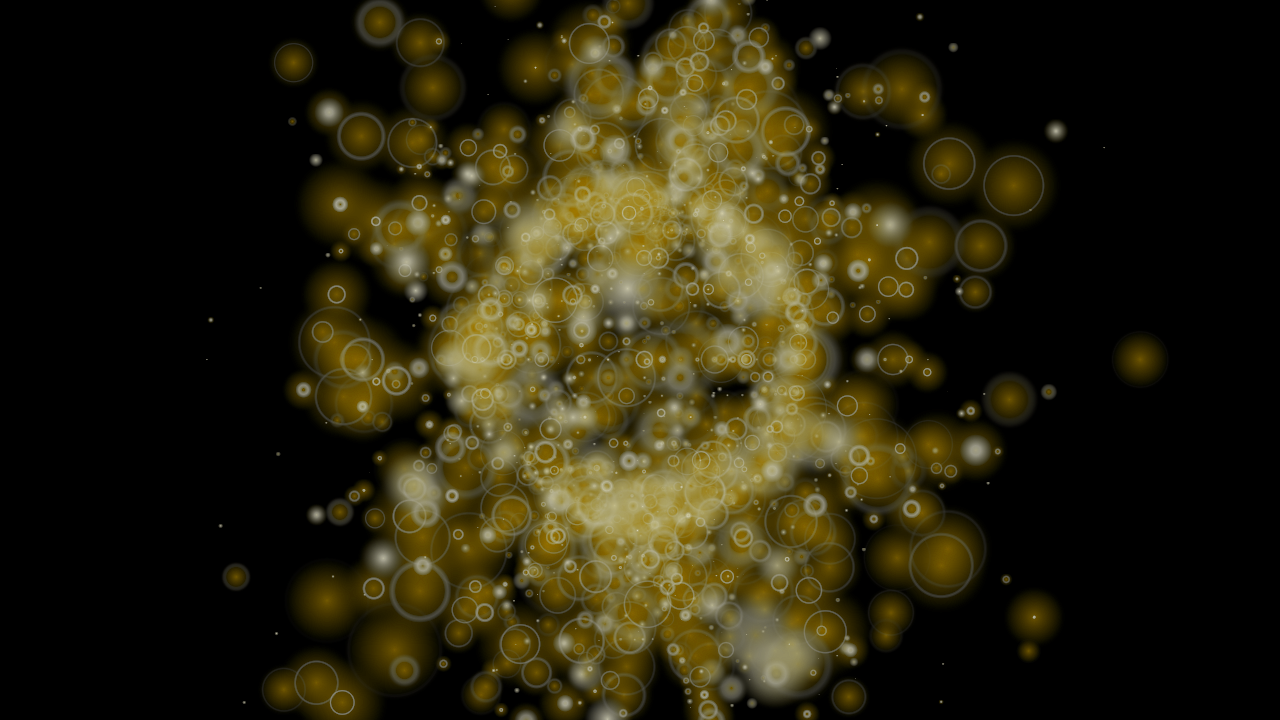
\includegraphics[trim=400 200 0 300,clip,width=\paperwidth]{4436.png}	%trimming relative to image size!
 %   \end{center}
%\end{figure}
%---------------------------------------------------------------------------------------
%	TITLE HEADLINE
%----------------------------------------------------------------------------------------
\vspace{-20.55pt}

%\begin{flushright}
	\hspace{-0.25\linewidth}\colorbox{bgcol}{\makebox[1.5\linewidth][c]{\HUGE{\textcolor{white}{Jan Küster} } \textcolor{sectcol}{\rule[-1mm]{1mm}{0.9cm}} \HUGE{ \textcolor{white}{Resume}}}}
%\end{flushright}

%---------------------------------------------------------------------------------------
%	TITLE HEADLINE
%----------------------------------------------------------------------------------------
\normalsize
\vspace{12pt}
\metasection{Languages:}Flex \& AIR, Java, Processing, Latex\\
\metasection{Concepts:}Requirements, Software Design, Design Pattern, Usability\\
\metasection{Activities:}FL Studio, Blender, Muay Thai, Grappling\\

\cvsection{Summary}\\
\vspace{-26pt}
\doublelist{Digital media graduate with three years of work experience as a software developer in the field of technology based assessment. Master classes were in teams from different disciplines and cultural backgrounds on (digital) solutions for complex problems. Specialized in development of test-scenario engines and innovative, rich media item formats. Prior knowledge has been collected in he field of usability / accessibility during bachelor studies.}

\cvsection{Education}\\
\cvevent{Master of Science Digital Media}{University of Bremen}\\
\cveventmeta{Title of the master thesis, usually a very long title for a very complex topic}{qrcode.png}\\
Lorem ipsum dolor sit amet, consectetur adipiscing elit. Donec a diam lectus. Sed sit amet ipsum mauris. \\

\cvevent{Bachelor of Science Digital Media}{University of Bremen}\\
\cveventmeta{Specialisation in usability}{qrcode.png}\\


\cvsection{Experience}


\cvevent{Poster Presentation}{DELFI}\\
\cveventmeta{Usability Guidelines for Tests with Functional Illiterates}{qrcode.png}\\
orem ipsum dolor sit amet, consectetur adipiscing elit. Donec a diam lectus. Sed sit amet ipsum mauris. Maecenas congue ligula ac quam viverra nec consectetur ante hendrerit. Donec et mollis dolor. Praesent et diam eget libero egestas mattis sit amet vitae augue. Nam tincidunt congue enim, ut porta lorem lacinia consectetur. \\


\cvevent{Technology Based Domain Specific Learning Assessment}{BMBF Project}\\
\cveventmeta{Scientific employee}{qrcode.png}\\
orem ipsum dolor sit amet, consectetur adipiscing elit. Donec a diam lectus. Sed sit amet ipsum mauris. Maecenas congue ligula ac quam viverra nec consectetur ante hendrerit. Donec et mollis dolor. Praesent et diam eget libero egestas mattis sit amet vitae augue. Nam tincidunt congue enim, ut porta lorem lacinia consectetur. \\











%
%\begin{flushleft}
%\begin{tikzpicture}
%\draw[help lines] (0,0) grid (9,9);
%\fill[orange] (1,1) circle (1);
%\end{tikzpicture}
%\end{flushleft} 

%
%\begin{multicols}{2} 
%\cvsection{Experience}
%\lorem\\
%\lorem\\
%\cvsection{Education}
%\lorem\\
%\lorem\\
%\end{multicols}



\end{document}